\subsection{Création du modèle}

Après avoir construit le corpus, nous pouvons passer à la création du modèle de traduction.
Dans cette section, nous allons détailler les étapes de sa construction.
La procédure d'entraînement est discutée dans la section suivante.

\subsubsection{Division du corpus}

Le corpus est divisé en trois parties : entraînement, validation et test.
La partie entraînement est utilisées pour optimiser les paramètres du modèle.
Cela peut conduire au phénomène de sur-apprentissage 
(où le modèle est bien ajusté aux données d'entraînement, mais ne généralise pas bien).
Pour détecter ce phénomène, nous utilisons la partie validation pour évaluer le modèle pendant l'entraînement.
La partie test est réservée pour l'évaluation finale du modèle (après l'entraînement).

\subsubsection{Tokenisation}

La création du modèle implique plusieurs choix techniques.
L'un des plus importants parmi ces choix est celui du tokeniseur.
Dans Section~\ref{subsec.nmt-transformer}, 
nous avons introduit le tokeniseur \gls{bpe}.
Nous avons décidé d'utiliser ce tokeniseur basé sur \gls{bpe} qui s'appelle ``\emph{WordPiece}''.
Il a été introduit par Google dans~\cite{Devlin_Chang_Lee_Touta11a_2019}.

Comme \gls{bpe}, WordPiece part d'un vocabulaire réduit à l'alphabet du corpus
puis, il l'élargit en fusionnant itérativement les tokens adjacents.
Contrairement à \gls{bpe}, la fusion n'est pas faite sur la base de la fréquence,
mais sur celle de la fonction d'évaluation suivante :
\begin{equation}
    \label{eq.wp-score}
    \mathrm{score}(x, y) = \frac{\prob{(x, y)}}{\prob{(x)} \prob{(y)}}
\end{equation}
où \(x\) et \(y\) sont deux tokens dans le vocabulaire à une itération donnée.

La division de la fréquence du couple par le produit de celles de ses composants
a pour but de défavoriser la fusion des tokens fréquents (qui sont souvent des mots).
Cela empêche la création de tokens plus longs qu'un mot et permet de conserver les tokens
qui représentent des affixes communs (comme ``im-'' et ``-able'').

Nous avons opté pour une taille de vocabulaire de 5000 tokens pour la source et la cible.
Des tokens spéciaux sont ajoutés au vocabulaire pour représenter la structure de la phrase.
Ces tokens sont :
\begin{itemize}
    \item \texttt{[BOS]} : début de la phrase ;
    \item \texttt{[EOS]} : fin de la phrase ;
    \item \texttt{[UNK]} : token inconnu (qui n'existe pas dans le vocabulaire) ;
    \item \texttt{[PAD]} : token de remplissage (utilisé pour ramener les phrases à la même longueur 
    dans le cas de l'entraînement par lots).
\end{itemize}

À la sortie du tokeniseur, une opération de \emph{numérisation} est effectuée.
Il s'agit d'une application bijective entre les tokens et les entiers (que nous appelons ``indices'').
Cela permet de représenter les phrases par des suites d'entiers de longueur variable.
Chose qui facilite leur représentation vectorielle.
Le fait qu'elle soit bijective permet de reconstruire les phrases 
à partir de ces suites d'entiers produites par le modèle.

\subsubsection{Représentation vectorielle des mots}

Comme discuté dans la Section~\ref{subsec.nmt-transformer},
un plongement lexical est appliqué après la tokenisation.
En effet, les indices retournés par le tokeniseur peuvent en principe être utilisés tels quels.
Cela présente en outre deux problèmes majeurs.
Le premier et que la plage des indices est aussi grande que la taille du vocabulaire.
Cela garantit que les mots de grands indices écrasent les autres lors de l'entraînement.
Le deuxième problème est que les indices ne sont pas structurés selon une quelconque relation sémantique.
Bien que d'être le plus souvent basés sur la fréquence des tokens, 
les indices ne contiennent pas d'information sur leur distribution conjointe.

Un plongement lexical est une application \(\Sigma \to \reals^d\) où \(\Sigma\) est le vocabulaire 
(qui passe le plus souvent par les indices) et \(d\) est la dimension du plongement (que nous avons fixé à 64).
Cela permet de remédier aux problèmes cités ci-dessus.
Le premier problème est résolu, car la norme des vecteurs de plongement peut être contrôlée.
Le deuxième est réglé, car les plongements, étant des vecteurs, présentent une structure vectorielle.
Il est possible de définir la similarité entre deux plongements en utilisant le produit scalaire.
Cela permet de capturer les relations sémantiques entre les tokens en s'assurant que les tokens corrélés
sont représentés par des vecteurs similaires (voir Figure~\ref{fig.embeddings}).

\begin{figure}[htb]
    \begin{center}
        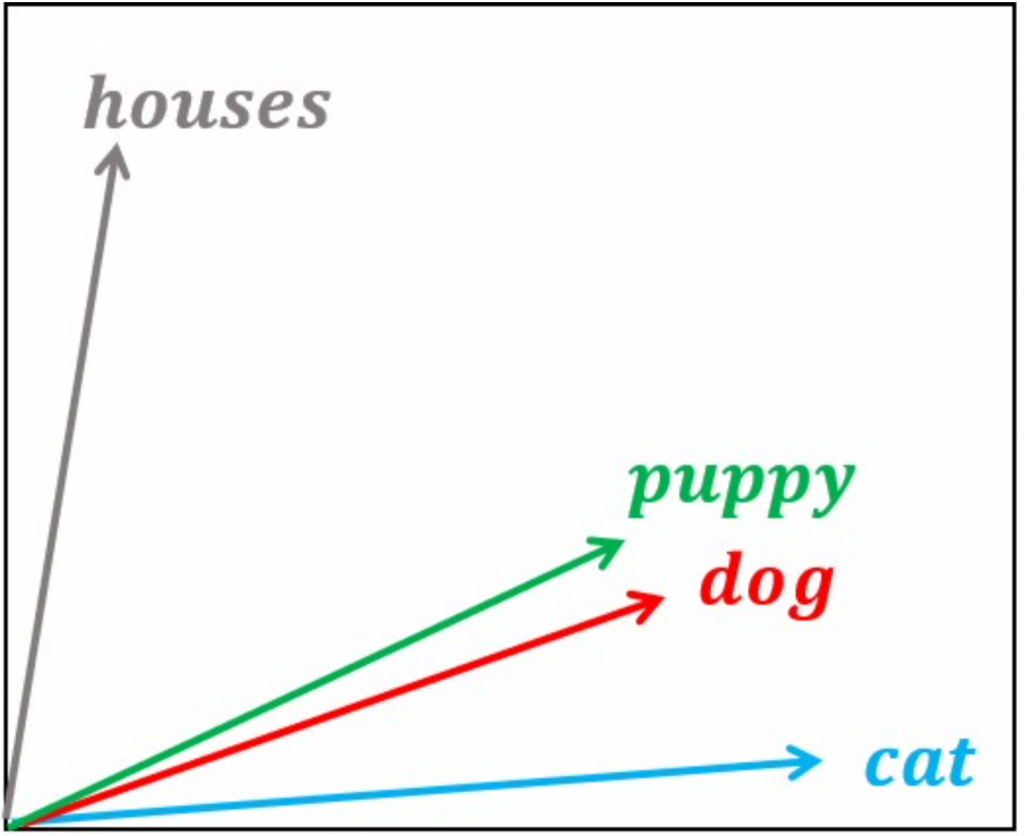
\includegraphics[width=8cm]{assets/images/embeddings.png}
    \end{center}
    \caption[Les plongements lexicaux de quelques mots de la langue anglaise.]%
    {Les plongements lexicaux de quelques mots de la langue anglaise \(d=2\).}
    \label{fig.embeddings}
\end{figure}

Plusieurs algorithmes existent pour calculer les plongements lexicaux (voir Section~\ref{subsec.nmt-transformer}).
Dans ce travail, nous utilisons une couche de plongement lexical simple.
Il contient un tableau de \(|\Sigma|\) vecteurs de dimension \(d\).
Elle est donc paramétrée par les composantes de ces vecteurs.
Cela donne une matrice de paramètres \(W\) dont les lignes sont les vecteurs de plongement :
\begin{equation}
    W = \overbrace{
    \begin{bmatrix}
        w_{11} & w_{12} & \cdots & w_{1N}\\
        w_{21} & w_{22} & \cdots & w_{2N}\\
        \vdots & \vdots & \ddots & \vdots\\
        w_{d1} & w_{d2} & \cdots & w_{dN}\\
    \end{bmatrix}}^{d = 64}
    \left.\vphantom{
        \begin{bmatrix}
            w_{11} & w_{12} & \cdots & w_{1N}\\
            w_{21} & w_{22} & \cdots & w_{2N}\\
            \vdots & \vdots & \ddots & \vdots\\
            w_{d1} & w_{d2} & \cdots & w_{dN}\\
        \end{bmatrix}}\right\}N = 5000
\end{equation}
qui a donc \(|\Sigma| \times d = 5000 \times 64 = 320000\) paramètres.
Pour calculer le plongement d'un token \(x\) d'indice \(i\), il suffit de prendre la ligne \(i+1\) de \(W\).
La matrice \(W\) peut être optimisée comme n'importe quelle autre matrice de paramètres.
Cela permet d'apprendre les plongements lexicaux à partir des données~\cite{Paszke_et_al_2019}.


\subsubsection{Architecture du modèle}

Suite à l'étude bibliographique du Chapitre~\ref{chap.mt-and-asr}, 
nous avons choisi d'utiliser un transformeur comme architecture de base pour notre modèle.
Nous avons opté pour le transformeur de base décrit dans~\cite{attention}.

Notre modèle est composé de 3 couches d'encodeurs et de 3 couches de décodeurs.
Chaque couche a 4 têtes d'attention.
La dimension de toutes les couches est de 64
et la fonction \(\relu\) est utilisée comme fonction d'activation%
\footnote{\(\relu: \reals\to\reals, x\mapsto \max{(0, x)}\).}.
Pour l'encodage positionnel, nous avons choisi de l'apprendre plutôt que d'utiliser un encodage sinusoïdal
comme celui décrit dans~\cite{attention}.

% \begin{figure}[hbt]
%     \begin{center}
%         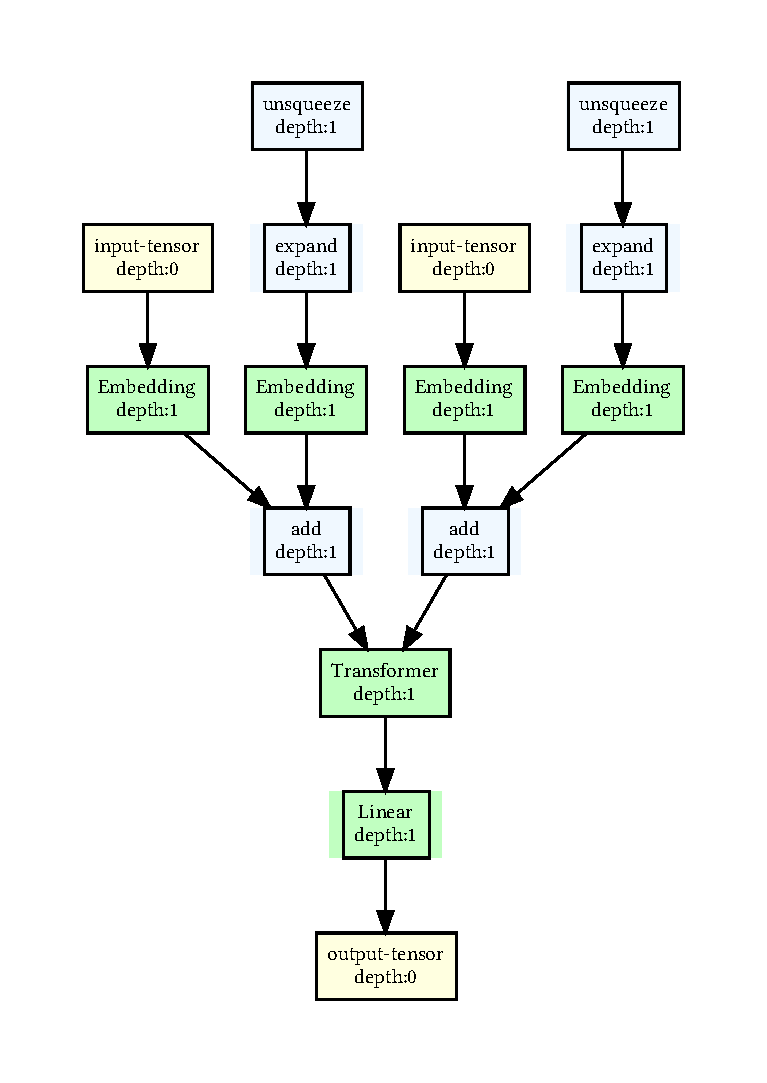
\includegraphics[height=\textwidth]{assets/pdf/model.pdf}
%     \end{center}
%     \caption{Architecture du modèle.}
%     \label{fig.model}
% \end{figure}